\section{Realization}
%Focus generale sulle tecnologie utilizzate
In this section we outline the technical aspects concerning the realization of our framework. Therefore we first present the enabler technologies through which we instantiate the design principles presented in \cref{sec:design}. After that, we discuss the interaction workflow between the instantiated technologies. Finally, we show the implementation details.
\begin{figure}[t]
\centering
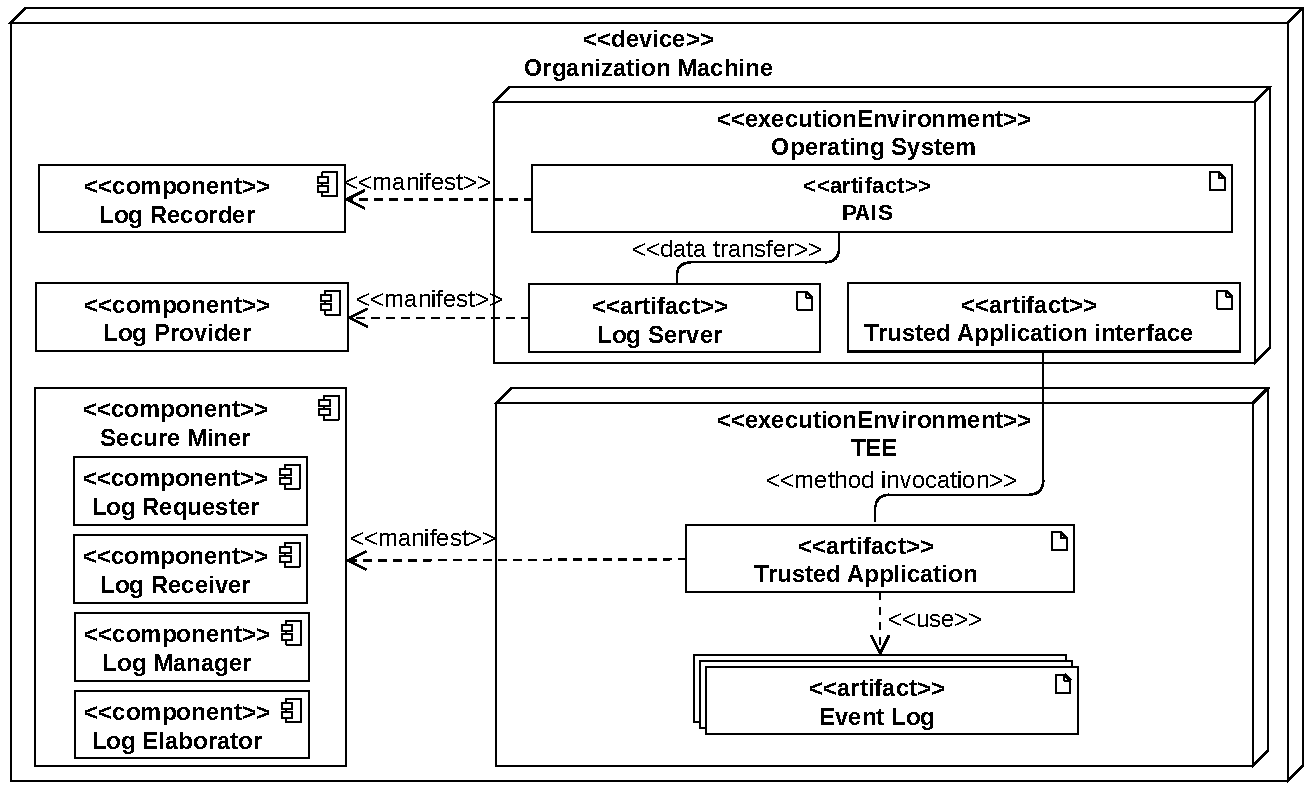
\includegraphics[width=10cm]{content/figures/deployment_diagram.pdf}
\caption{UML deployment diagram.}
\label{fig:deployment_diagram}
\end{figure}
\subsection{Deployment}
As follow, we bridge the gap between high-level system architecture and its practical realization. \cref{fig:deployment_diagram} depicts a \textit{UML deployment diagram} \cite{koch2002expressive} that aims to help with understanding the instantiated infrastrucuture. 

The \texttt{Organization Machine} represent the physical computation \textit{device} embracing the software and hardware entities of the company. The \texttt{Log Recorder}, the \texttt{Log Provider} and \texttt{Secure Miner} are included in the \texttt{Organization Machine} as abstract \textit{components} . These logical elements incorporate the core functionalities already discussed in \cref{sec:design}. The \texttt{Organization Machine} is characterized by two \textit{execution environment}s namely the \texttt{Operative System} and the \texttt{Trusted Execution Environment}.

Software entities that we expose to the users of the \texttt{Organization Machine} run inside the \texttt{Operative System}. We mainfest the functionalities offered by the \texttt{Log Recorder} in the \texttt{Process Aware Information System}  \cite{Dumas.etal/2018:FundamentalsofBPM}. These systems help users to handle business processes including accounting and resource management. In our solution, the \texttt{Process-Aware Information System} provides the \texttt{Log Server} access to event logs. \texttt{Log Servers} are web services which processes remote data request and provides event log to miners. We build this entities upon existing web standards such as HTTP, FTP and Goopher.

\texttt{Trusted Execution Environment}s are the core technologies of our solution. It creates a separated context from the normal \texttt{Operating System} to protect code and data through hardware-based security features in a reserved zone of the \texttt{Organization Machine}'s CPU. We leverage the isolation guarantees offered by this techonologies to instantiate a \texttt{Trusted Application} to fulfill the functionalities of the \texttt{Secure Miner} and its subcomponents.
%What the secure miner can do
%-TEEs ensure that the code and data executed within the environment are protected from unauthorized access
%TEEs provide mechanisms to protect sensitive data stored within the environment. Encryption and decryption operations can be performed securely without exposing the data to the less secure parts of the system.
%


%The \texttt{PAIS Interface} collects the logic to interact with the Process-aware Information Sytem (\texttt{PAIS}) of the \texttt{Organization}. \texttt{PAIS} systems help \texttt{Organization}s to handle business processes including accounting and resource management. The maintenance of event logs is the core tasks performed by these systems~\cite{Dumas.etal/2018:FundamentalsofBPM}. In our architecture, we generalize the interaction with \texttt{PAIS}s through the \texttt{PAIS Interface}. The \texttt{PAIS Interface} is queried by the local \texttt{Log Provider} for event logs to be fed into \texttt{Secure Miner}s.

\subsection{Workflow}
\subsection{Implementation}
%\subsubsection{Event Log Generation}
%Tecnologie utilizzate
%Sintesi del processo di generazione dei log
%\subsubsection{Trusted Miner and Log Provider}
%Tecnologia TEE usata
%Linguaggio usato per programmare in TEE
%Algoritmo implementato
%Rappresentazioni intermedie (PNML, Petrinet, ecc...)
%Linguaggio Log provider
